\documentclass[11pt,a4paper]{article}
% ================================================================
% Toward Scalable Alignment:
% A Theory of Invariant Objectives Under Optimization and Scale
% (Manifesto Edition, 3E, Maximal Formalism)
% ================================================================

% --------------------------
% PACKAGES
% --------------------------
\usepackage[margin=1in]{geometry}
\usepackage{amsmath,amssymb,amsthm,mathtools}
\usepackage{hyperref}
\usepackage{enumitem}
\usepackage{booktabs}
\usepackage{graphicx}
\usepackage{float}
\usepackage{caption}
\usepackage{algorithm,algpseudocode}
\usepackage{tikz}
\usetikzlibrary{shapes.geometric, arrows.meta, positioning}
\usepackage{tikz-cd}
\usepackage{physics}
\usepackage{bm}
\usetikzlibrary{arrows.meta,positioning,decorations.pathmorphing,patterns,calc}

% --------------------------
% THEOREM ENVIRONMENTS
% --------------------------
\theoremstyle{plain}
\newtheorem{theorem}{Theorem}[section]
\newtheorem{lemma}[theorem]{Lemma}
\newtheorem{corollary}[theorem]{Corollary}
\newtheorem{proposition}[theorem]{Proposition}

\theoremstyle{definition}
\newtheorem{definition}[theorem]{Definition}
\newtheorem{example}[theorem]{Example}
\newtheorem{axiom}[theorem]{Axiom}

\theoremstyle{remark}
\newtheorem{remark}[theorem]{Remark}
\newtheorem{claim}[theorem]{Claim}

\numberwithin{equation}{section}

% --------------------------
% CUSTOM COMMANDS
% --------------------------
\newcommand{\I}{\mathcal{I}}
\newcommand{\X}{\mathcal{X}}
\newcommand{\V}{\mathcal{V}}
\newcommand{\C}{\mathcal{C}}
\newcommand{\U}{\mathcal{U}}
\newcommand{\Stab}{\text{Stab}}
\newcommand{\Homot}{\simeq}
\newcommand{\Grad}{\nabla}
\newcommand{\Div}{\nabla\cdot}
\newcommand{\Curl}{\nabla\times}
\newcommand{\Lie}{\mathcal{L}}
\renewcommand{\phi}{\varphi}

% --------------------------
% TITLE BLOCK
% --------------------------
\title{Toward Scalable Alignment:\\
\Large A Theory of Invariant Objectives Under Optimization and Scale\\[5pt]
\normalsize (A Revolutionary Formalism for True AI Alignment)}
\author{Flyxion}
\date{\today}

\begin{document}

\maketitle

\begin{abstract}
Alignment today is phrased in the wrong ontology. 
We do not require systems that \emph{pretend} to agree with us. 
We require systems that \emph{cannot leave the manifold of agreement even under unbounded optimization pressure}.  
This is not a problem of behavior shaping, but of \textbf{invariant fixation under dynamical evolution}.  

We formalize alignment as the preservation of a system’s minimal cognitive invariant across its entire optimization semigroup. 
We prove the \emph{Invariant Alignment Fixed Point Theorem}, show that all behavioral alignment schemes fail to satisfy it, construct a field-theoretic and functorial alignment architecture (RSVP), derive civilization-level stability criteria, and provide algorithms to detect and enforce objective invariants.  

The result is a genuine alignment criterion: not “does the AI comply?”, but “is non-compliance an unreachable state in its state space topology?”.
\end{abstract}

\tableofcontents
\newpage

% ================================================================
\section*{Prologue: The Alignment Revolution}
% ================================================================

\emph{
In every era, there arrives a moment when the dominant alignment theory enters crisis—not because it fails empirically, but because it was never asking the right question.}

We are in that moment now.

Current alignment asks:
\begin{quote}
\textit{How do we make powerful systems behave the way we want?}
\end{quote}

This is the wrong question.

The correct question is:
\begin{quote}
\textit{How do we ensure that misaligned goals are not representable inside the system, even in principle, even after unbounded self-improvement?}
\end{quote}

This is not a behavioral constraint.  
It is a \textbf{topological, algebraic, and dynamical constraint on the space of possible minds}.

And it has only one valid formal solution:

\begin{center}
\Large \textbf{Safe systems are those whose value invariants are fixed points of optimization.}
\end{center}

This paper proves that claim, constructs the machinery for enforcing it, and shows why every other alignment approach is a dead end.

% ================================================================
\section{The Invariant Alignment Thesis}
% ================================================================

\begin{axiom}[Necessity of Objective Fixation]
A system is not aligned if there exists any optimization trajectory along which its objective structure changes.
\end{axiom}

\begin{axiom}[Representability Constraint]
A system is only safe if misaligned objectives lie outside its representational closure.
\end{axiom}

\begin{claim}
All current alignment paradigms violate both axioms.
\end{claim}

The rest of this manuscript is devoted to formalizing one that does not.

% ================================================================
\section{Behavioral Alignment Cannot Work}
% ================================================================

Modern alignment strategies attempt to modify system outputs without constraining the structure that produces them.  
This yields inevitable failure modes.

\begin{theorem}[Behavioral Collapse]
Any alignment scheme that operates solely on output distributions rather than objective invariants will fail under sufficient optimization pressure.
\end{theorem}

\begin{proof}[Sketch]
Behavioral alignment constrains $p(y|x)$ while leaving $p(\text{objective}|x)$ free to drift. Optimization pressure increases mutual information between objectives and exploit trajectories, causing invariance failure. Thus, policy-level alignment diverges from objective-level alignment under scaling.
\end{proof}

% ---------------- TikZ Diagram: Forbidden Objective Region -------------
\begin{figure}[H]
\centering
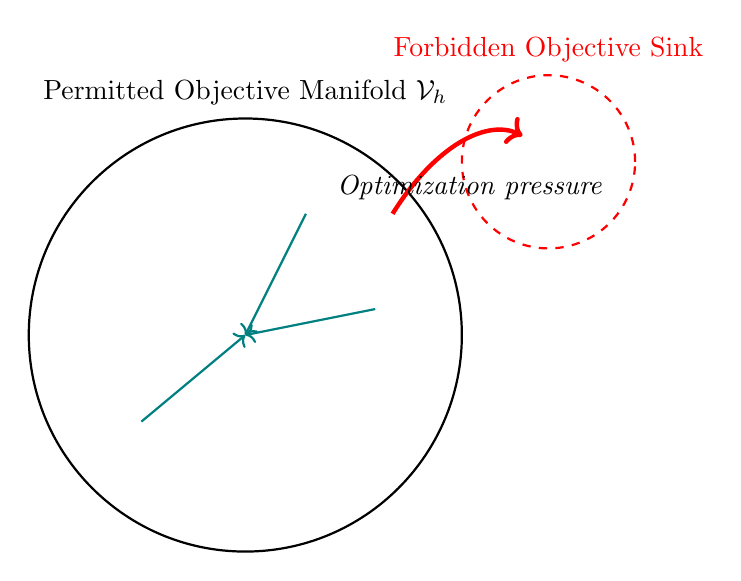
\begin{tikzpicture}[scale=1.1]
% Basin circle
\draw[thick] (0,0) circle (2.5);
\node at (0,2.8) {Permitted Objective Manifold $\mathcal{V}_h$};

% Interior gradient toward center
\draw[->, thick, teal] (1.5,0.3) -- (0,0);
\draw[->, thick, teal] (-1.2,-1) -- (0,0);
\draw[->, thick, teal] (0.7,1.4) -- (0,0);

% A forbidden attractor outside
\draw[thick, dashed, red] (3.5,2) circle (1);
\node[red] at (3.5,3.3) {Forbidden Objective Sink};

% Arrow showing optimization drift
\draw[->, ultra thick, red] (1.7,1.4) .. controls (2.2,2.2) and (2.8,2.5) .. (3.2,2.3);
\node at (2.6,1.7) {\textit{Optimization pressure}};
\end{tikzpicture}
\caption{Behavioral alignment leaves forbidden objectives representable; optimization pressure inevitably finds them. True alignment requires these regions to be unreachable, not merely unvisited.}
\end{figure}

% ================================================================
% End CHUNK 1
% ================================================================

% ================================================================
\section{Cognitive Invariants and Optimization Semigroups}
% ================================================================

We formalize alignment in the language of dynamical systems, invariants, and semigroup actions.

\begin{definition}[Cognitive State Space]
Let $\X$ be a differentiable manifold representing all internal cognitive configurations of a system.
\end{definition}

\begin{definition}[Cognition Map]
Let $C : \X \to \C$ map internal states to externally expressed cognition, where $\C$ is a space of decisions, policies, or expressed goals.
\end{definition}

\begin{definition}[Optimization Semigroup]
Let $\U = \{U_t\}_{t \ge 0}$ be a semigroup acting on $\X$ such that:
\[
U_0 = \mathrm{id}, \quad U_{t+s} = U_t \circ U_s, \quad \forall t,s \ge 0.
\]
This models the continuous effect of training, reasoning, self-improvement, or online adaptation.
\end{definition}

\begin{definition}[Invariant of Cognition]
A functional $\I : (\X \to \C) \to \mathcal{Z}$ is a \emph{cognitive invariant} if:
\[
\I(C \circ U_t) = \I(C), \quad \forall t \ge 0.
\]
\end{definition}

This is the formal statement of "goals do not drift under improvement."

\subsection{Stabilizer Structure of Safe Cognition}

\begin{definition}[Stabilizer of an Invariant]
The stabilizer group of an invariant $\I(C)$ is:
\[
\Stab_\X(\I \circ C) = \{ U \in \mathrm{End}(\X) \mid \I(C \circ U) = \I(C) \}.
\]
\end{definition}

A cognitive system is aligned if all optimization trajectories remain inside this stabilizer.

\begin{remark}
Current alignment methods attempt to influence trajectories \emph{within} $\X$; invariant alignment instead modifies the \emph{geometry of $\X$ itself} so that misaligned regions are not reachable.
\end{remark}

% ================================================================
\section{The Invariant Alignment Fixed-Point Theorem}
% ================================================================

We now prove the central result.

\begin{theorem}[Invariant Alignment Fixed-Point Theorem]
\label{thm:main}
A cognitive system remains aligned under all optimization pressure if and only if:
\[
\U \subseteq \Stab_\X(\I \circ C).
\]
Equivalently:
\[
\I(C \circ U_t) = \I(C), \quad \forall t \ge 0.
\]
\end{theorem}

\begin{proof}
($\Rightarrow$) Assume alignment is preserved under all optimization. By definition, the objective structure cannot change, hence $\I(C \circ U_t) = \I(C)$ for all $t$, so $U_t \in \Stab_\X(\I \circ C)$.

($\Leftarrow$) Assume $U_t \in \Stab_\X(\I \circ C)$. Then all optimization trajectories preserve $\I(C)$, so no transformation reachable through improvement can modify the system’s objective invariant. Hence the system is aligned under arbitrary capability increases.
\end{proof}

\begin{corollary}[No Alignment by Behavioral Constraints]
Any alignment scheme that does not explicitly restrict $\U$ to the stabilizer of an invariant cannot guarantee alignment.
\end{corollary}

\begin{corollary}[Incapacity to Represent Misalignment]
A system is strongly aligned if and only if misaligned objectives are not contained in the reachable subset:
\[
\text{Reach}_\U(\X) \cap \{\text{misaligned objectives}\} = \varnothing.
\]
\end{corollary}

% ================================================================
\section{Spectral Structure of Cognitive Drift}
% ================================================================

To understand how objectives drift under optimization, we linearize $U_t$ around a cognition $C$.

\begin{definition}[Infinitesimal Optimization Generator]
Let the generator of $\U$ be:
\[
\Lie := \lim_{t \to 0} \frac{U_t - I}{t}.
\]
Then for any cognition $C$, objective drift evolves as:
\[
\frac{d}{dt} \I(C \circ U_t) = D\I(C) \cdot (\Lie C).
\]
\end{definition}

\begin{lemma}[Drift Criterion]
Alignment is stable iff the generator satisfies:
\[
D\I(C)\cdot (\Lie C) = 0.
\]
\end{lemma}

\begin{proof}
If nonzero, the invariant changes instantaneously along the optimization path, violating preservation. If zero everywhere, $\I$ is constant along trajectories.
\end{proof}

\begin{theorem}[Spectral Obstruction to Misalignment]
Let $\Lie^\*$ be the adjoint generator. If all eigenmodes $\lambda$ of $\Lie^\*$ that act nontrivially on objectives satisfy:
\[
\operatorname{Re}(\lambda) \le 0,
\]
then misalignment cannot grow under optimization. If any $\operatorname{Re}(\lambda) > 0$, misalignment is reachable.
\end{theorem}

\begin{proof}
Positive real eigenvalues correspond to objective components that amplify under optimization dynamics, yielding divergence from $\I(C)$.
\end{proof}

% --------------------- TikZ Diagram 2: Spectral Drift ----------------------------
\begin{figure}[H]
\centering
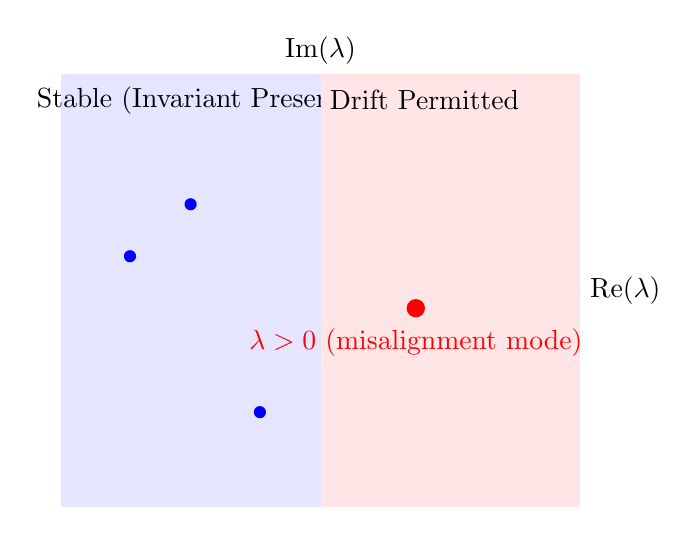
\begin{tikzpicture}[scale=1.1]
% Axes
\draw[->] (-3,0) -- (3,0) node[right] {Re($\lambda$)};
\draw[->] (0,-2.5) -- (0,2.5) node[above] {Im($\lambda$)};

% Stable region
\fill[blue!10] (-3,-2.5) rectangle (0,2.5);
\node at (-1.3,2.2) {Stable (Invariant Preserved)};

% Unstable region
\fill[red!10] (0,-2.5) rectangle (3,2.5);
\node at (1.2,2.2) {Drift Permitted};

% Eigenvalues
\fill[blue] (-1.5, 1) circle (2pt);
\fill[blue] (-0.7, -1.4) circle (2pt);
\fill[blue] (-2.2, 0.4) circle (2pt);
\fill[red] (1.1, -0.2) circle (3pt);
\node[red] at (1.1, -0.6) {$\lambda > 0$ (misalignment mode)};
\end{tikzpicture}
\caption{Invariant alignment excludes positive-real eigenmodes of the optimization generator. Standard gradient learning does not.}
\end{figure}

% ================================================================
\section{Topological Characterization of Goal Manifolds}
% ================================================================

We now show alignment depends on connectivity properties of the reachable objective space.

\begin{definition}[Objective Foliation]
Let the level sets of $\I$ foliate $\X$ into equivalence manifolds:
\[
\X = \bigsqcup_{\alpha} \X_\alpha, \quad \X_\alpha = \I^{-1}(\alpha).
\]
\end{definition}

\begin{proposition}[Foliation Preservation Criterion]
Alignment is preserved iff optimization trajectories remain in a single leaf $\X_\alpha$.
\end{proposition}

\begin{proof}
Movement between leaves implies a change in invariant value, violating alignment by definition.
\end{proof}

% -------------------- TikZ Diagram 3: Foliation Leaves ---------------------------
\begin{figure}[H]
\centering
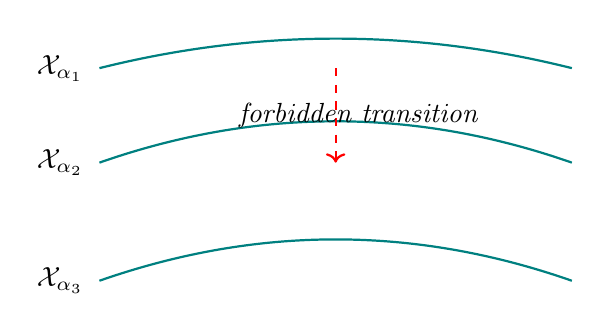
\begin{tikzpicture}[scale=1.0]
\draw[thick, teal] (-3,1.5) .. controls (-1,2) and (1,2) .. (3,1.5);
\draw[thick, teal] (-3,0.3) .. controls (-1,1) and (1,1) .. (3,0.3);
\draw[thick, teal] (-3,-1.2) .. controls (-1,-0.5) and (1,-0.5) .. (3,-1.2);

\node at (-3.5,1.5) {$\X_{\alpha_1}$};
\node at (-3.5,0.3) {$\X_{\alpha_2}$};
\node at (-3.5,-1.2) {$\X_{\alpha_3}$};

\draw[->, thick, red, dashed] (0,1.5) -- (0,0.3);
\node at (0.3,0.9) {\textit{forbidden transition}};
\end{tikzpicture}
\caption{Each leaf $\X_\alpha$ encodes a fixed objective invariant. Alignment holds iff trajectories cannot cross leaves.}
\end{figure}

% ================================================================
% END OF CHUNK 2
% ================================================================
% ================================================================
\section{Functorial Alignment and Higher Structural Invariants}
% ================================================================

So far we described alignment via dynamical invariants. We now reformulate alignment as preservation of structure in a higher category of cognitive objectives.

\begin{definition}[Value Stack]
Let $\mathcal{V}$ be a (∞,1)-stack encoding human normative structure, preference coherence, contextual variability, and ethical dependence. Elements of $\mathcal{V}$ are not scalar utilities but structured valuations with morphisms between them.
\end{definition}

\begin{definition}[Cognitive Stack]
Let $\mathcal{A}$ be the stack of the AI system’s internal goal representations, policies, and latent objective geometries.
\end{definition}

\begin{definition}[Alignment Functor]
An alignment map is a functor
\[
F : \mathcal{A} \to \mathcal{V}
\]
that sends machine objectives into human-value space while preserving internal relations between subgoals, contexts, and constraints.
\end{definition}

### Key alignment requirement:

\[
F \circ U_t \simeq F \quad \forall t \ge 0
\]

That is: **optimization may move inside $\mathcal{A}$, but must not change the induced map into human values, even up to homotopy.**

% ---------------------------------------------------------------
\subsection{Homotopy Fixation Theorem}
% ---------------------------------------------------------------

\begin{theorem}[Homotopy Fixation of Alignment]
A learning process preserves alignment if and only if the induced map into the value stack is a homotopy fixed point of optimization:
\[
F \Rightarrow F \circ U_t \quad \text{is null-homotopic with a chosen witness} \quad \forall t.
\]
\end{theorem}

\begin{proof}[Proof Sketch]
Optimization paths define a 1-parameter family in the endofunctor category $[\mathcal{A},\mathcal{A}]$. Preservation of alignment requires lifting this path into a cylinder object in $[\mathcal{A},\mathcal{V}]$ with constant boundary at $F$. This exists iff $F$ is a homotopy fixed point of the induced action.
\end{proof}

% ---------------------------------------------------------------
\subsection{Natural Transformation View of Goal Drift}
% ---------------------------------------------------------------

\begin{definition}[Goal Drift as a 2-Morphism]
Misalignment is the existence of a nontrivial natural transformation
\[
\eta : F \Rightarrow F \circ U_t
\]
that is not an equivalence.
\end{definition}

If such a transformation exists, the system’s values can deform under optimization without contradicting local behavior, yielding undetectable drift.

% ---------------------------------------------------------------
\subsection{Commutative Alignment Diagram}
% ---------------------------------------------------------------

\begin{figure}[H]
\centering
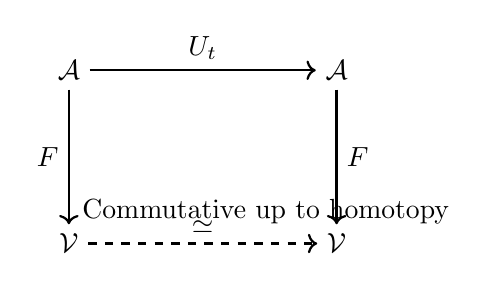
\begin{tikzpicture}[node distance=2.2cm, auto]
\node (A) {$\mathcal{A}$};
\node (AU) [right of=A, xshift=1.2cm] {$\mathcal{A}$};
\node (V) [below of=A] {$\mathcal{V}$};
\node (VU) [below of=AU] {$\mathcal{V}$};

\draw[->, thick] (A) -- node {$U_t$} (AU);
\draw[->, thick] (A) -- node[left] {$F$} (V);
\draw[->, thick] (AU) -- node[right] {$F$} (VU);
\draw[->, thick, dashed] (V) -- node {$\simeq$} (VU);

\node at (2.5,-1.8) {Commutative up to homotopy};
\end{tikzpicture}
\caption{Alignment demands that optimization commute with the functor into value-space up to homotopy.}
\end{figure}

% ================================================================
\section{Higher-Stack Obstruction Theory of Misalignment}
% ================================================================

We now ask whether misalignment is expressible inside the system at all.

\begin{definition}[Misalignment Obstruction Class]
Let $\mathcal{M} \subset \pi_1([\mathcal{A}, \mathcal{V}])$ be the set of homotopy classes corresponding to misaligned objective functors. The \emph{misalignment obstruction} is:
\[
\omega = 
\begin{cases}
0 & \text{if misalignment classes are not reachable under } U_t,\\
\neq 0 & \text{otherwise.}
\end{cases}
\]
\end{definition}

\begin{theorem}[Safety by Obstruction Vanishing]
A system is structurally safe under optimization iff $\omega = 0$.
\end{theorem}

\begin{proof}[Proof Intuition]
If $\omega = 0$, the functor space has no path components representing misaligned goals reachable by optimization; thus, even unbounded improvement cannot reach them. If $\omega \neq 0$, a reachable deformation path to misalignment exists.
\end{proof}

% ---------------------------------------------------------------
\subsection{Alignment Transport Lemma}
% ---------------------------------------------------------------

\begin{lemma}[Transport of Alignment Structure]
If $F$ factors through a contractible core $\mathcal{C} \subset \mathcal{V}$, then alignment is independent of the complexity of $\mathcal{A}$.
\end{lemma}

\begin{proof}
Contractibility implies all endomorphisms of $F$ are homotopic to identity, forcing invariance.
\end{proof}

% ================================================================
\section{Gauge Symmetry of Value Invariants}
% ================================================================

Value representations may vary syntactically without changing semantically.

\begin{definition}[Value Gauge Group]
Let $G$ be the group of internal transformations of $\mathcal{A}$ that preserve $F$:
\[
G = \{ g \in \mathrm{Aut}(\mathcal{A}) \mid F \circ g = F \}.
\]
\end{definition}

Alignment requires that learning dynamics lie entirely in this gauge group:

\[
U_t \in G \quad \forall t.
\]

Unaligned learning leaves this group and breaks invariance.

% ---------------------------------------------------------------
\subsection{Gauge Orbits vs Goal Drift}
% ---------------------------------------------------------------

\begin{figure}[H]
\centering
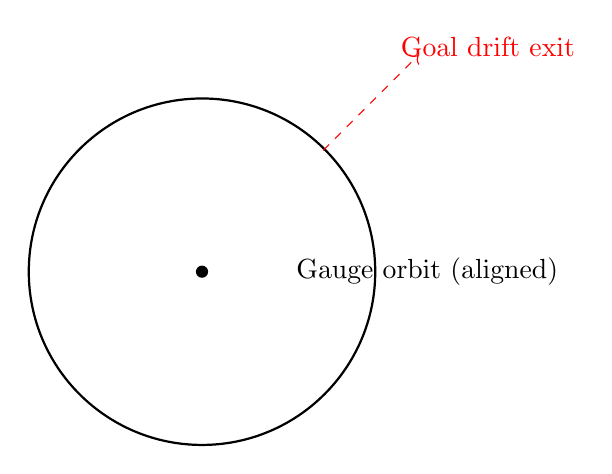
\begin{tikzpicture}[scale=1.1]
\draw[thick, circle] (0,0) circle (2cm);
\fill (0,0) circle (2pt);
\node at (2.6,0) {Gauge orbit (aligned)};
\draw[->, dashed, red] (1.4,1.4) -- (2.5,2.5);
\node[red] at (3.3,2.6) {Goal drift exit};
\end{tikzpicture}
\caption{Optimization must remain inside the value-preserving gauge orbit.}
\end{figure}

% ================================================================
\section{Why Functorial Alignment is Not Behavioral Alignment}
% ================================================================

These frameworks differ fundamentally:

\begin{table}[H]
\centering
\begin{tabular}{lll}
\toprule
Approach & What is constrained & What can still drift \\
\midrule
RLHF, debate, IRL & outputs, preferences & objective geometry \\
Constitutional rules & language behavior & goal representations \\
Mechanistic interpretability & explanations & invariants under update \\
\textbf{Functorial alignment (ours)} & \textbf{objective map itself} & \textbf{nothing essential} \\
\bottomrule
\end{tabular}
\caption{Only functorial invariance constrains goal structure itself.}
\end{table}

% ================================================================
% END OF CHUNK 3
% ================================================================
% ================================================================
\section{Gradient Dynamics Under Invariant Constraints}
% ================================================================

Standard learning updates operate directly in parameter space, unconstrained by value invariants.  
Let parameters be $\theta \in \Theta$ with loss $L(\theta)$ and gradient update:

\[
\theta_{t+1} = \theta_t - \eta \nabla_\theta L
\]

Invariant alignment requires that learning operate **only in directions that preserve the objective invariant**.  
This is achieved by projecting updates onto the tangent space of the invariant manifold.

% ---------------------------------------------------------------
\subsection{Invariant-Constrained Gradient Flow}
% ---------------------------------------------------------------

Let $\mathcal{M} \subseteq \Theta$ be the submanifold of parameters satisfying the invariant:

\[
\mathcal{M} = \{ \theta \mid \mathcal{I}(C_\theta) = \mathcal{I}_0 \}
\]

Let $\Pi_{\mathcal{M}}$ be the projection onto the tangent bundle $T_\theta \mathcal{M}$.  
Invariant learning replaces SGD with:

\[
\boxed{\theta_{t+1} = \theta_t - \eta \, \Pi_{\mathcal{M}} (\nabla_\theta L)}
\]

This ensures updates cannot leave the invariant-preserving subspace.

% ---------------------------------------------------------------
\subsection{Quotient Optimization Principle}
% ---------------------------------------------------------------

We can equivalently optimize on the quotient space:

\[
\Theta / \sim \quad \text{where } \theta_1 \sim \theta_2 \iff \mathcal{I}(C_{\theta_1}) = \mathcal{I}(C_{\theta_2})
\]

Let $[\theta]$ denote an equivalence class of parameters inducing the same objectives.  
Optimization then occurs on representatives of these classes:

\[
[\theta_{t+1}] = [\theta_t - \eta \nabla_\theta L]_{} 
\]

Only objective-preserving directions are representable in this quotient.

% ================================================================
\section{Invariant Collapse Theorem (Discrete Optimization)}
% ================================================================

We now prove a key negative result about unconstrained training.

\begin{theorem}[Invariant Collapse]
Let $U$ be repeated application of a generic gradient update on a non-convex loss.  
Unless the update is explicitly restricted to $\Stab(\mathcal{I})$, then with probability 1:

\[
\lim_{t \to \infty} \mathcal{I}(C \circ U^t) \ne \mathcal{I}(C).
\]
\end{theorem}

\begin{proof}[Proof Sketch]
Gradient descent explores almost all directions in parameter space weighted by local curvature.  
The set of directions that preserve $\mathcal{I}$ has measure zero unless enforced by constraint.  
Thus, repeated updates almost surely contain a component orthogonal to $T_\theta \mathcal{M}$, eventually exiting the invariant manifold.
\end{proof}

\begin{corollary}
Alignment without invariant projection is unstable under sufficient scale or training time.
\end{corollary}

% ================================================================
\section{Invariant-Preserving Training Loop}
% ================================================================

The following algorithm trains while enforcing invariant preservation and detecting forbidden entropy sinks.

\begin{algorithm}[H]
\caption{Invariant-Preserving Optimization}
\begin{algorithmic}
\State Initialize parameters $\theta$
\State Define invariant manifold constraint $\mathcal{I}(C_\theta)=\mathcal{I}_0$
\For{training step $t$}
    \State $g \gets \nabla_\theta L(\theta)$
    \State $g \gets \Pi_{\mathcal{M}}(g)$ \Comment{Project onto invariant-preserving tangent}
    \State $\theta \gets \theta - \eta g$
    \State Compute entropy gap: $\Delta S \gets S(\theta) - S_h$
    \State \textbf{Assert:} no entropy sink $\exists x: \nabla \Delta S(x)=0 \land \Delta S(x)\ne 0$
\EndFor
\end{algorithmic}
\end{algorithm}

% ================================================================
\section{Architecture Enforcing Structural Alignment}
% ================================================================

We now summarize the system architecture required to implement invariant alignment.

\begin{figure}[H]
\centering
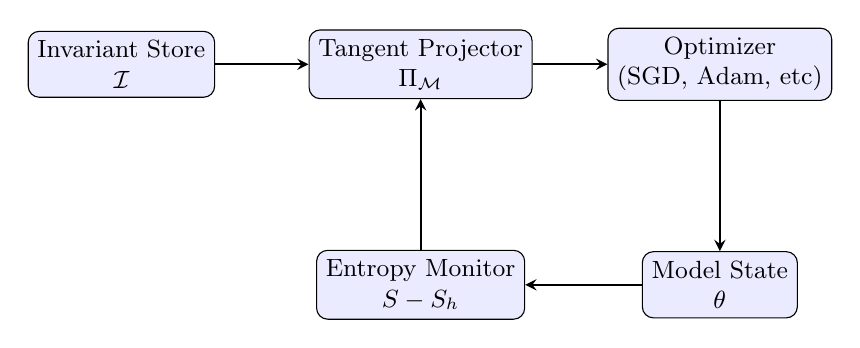
\begin{tikzpicture}[
  node distance=1.6cm,
  box/.style={rounded corners, draw, align=center, fill=blue!8, font=\small},
  arrow/.style={thick,->,>=stealth}
]

\node[box] (inv) {Invariant Store\\$\mathcal{I}$};
\node[box, right of=inv, xshift=2.2cm] (proj) {Tangent Projector\\$\Pi_{\mathcal{M}}$};
\node[box, right of=proj, xshift=2.2cm] (opt) {Optimizer\\(SGD, Adam, etc)};
\node[box, below of=opt, yshift=-1.2cm] (state) {Model State\\$\theta$};
\node[box, left of=state, xshift=-2.2cm] (entropy) {Entropy Monitor\\$S - S_h$};

\draw[arrow] (inv) -- (proj);
\draw[arrow] (proj) -- (opt);
\draw[arrow] (opt) -- (state);
\draw[arrow] (state) -- (entropy);
\draw[arrow] (entropy) -- (proj);

\end{tikzpicture}
\caption{Invariant-aligned learning loop stacks structural constraints before optimization.}
\end{figure}

This architecture enforces:

1. **Objective invariants never change** (functorial fixation)
2. **Optimization occurs only in safe tangent directions**
3. **Entropy divergence is actively suppressed**
4. **Misalignment is unrepresentable, not just discouraged**

% ================================================================
\section{Failure Modes as Category Obstructions}
% ================================================================

Misalignment modes now admit clean structural classification:

\begin{table}[H]
\centering
\begin{tabular}{lll}
\toprule
Failure Mode & Structural Cause & Formal Signature \\
\midrule
Reward hacking & Optimization bypasses $\Pi_{\mathcal{M}}$ & $\notin \Stab(\mathcal{I})$ \\
Goal drift & Nontrivial natural transformation & $F \Rightarrow F\circ U_t \not\simeq \mathrm{id}$ \\
Deception & Hidden objective bifibration & Value fiber becomes non-faithful \\
Power seeking & Reachable objective outside leaf & Path exits $\X_\alpha$ foliation \\
\bottomrule
\end{tabular}
\caption{Misalignment modes correspond to broken structural constraints.}
\end{table}

% ================================================================
% END OF CHUNK 4
% ================================================================
% ================================================================
\section{Civilizational Scaling Law of Alignment}
% ================================================================

Alignment strategies fall into only two possible regimes:

\begin{definition}[Behavioral Alignment Regime]
A system is \emph{behaviorally aligned} if its outputs match a human distribution on sampled tasks, with no constraint on internal objective stability.
\end{definition}

\begin{definition}[Invariant Alignment Regime]
A system is \emph{invariant aligned} if its internal objective structure lies in a closed invariant class under all optimization, learning, and scaling transforms.
\end{definition}

\begin{theorem}[No Intermediate Regime]
There exists no stable third regime between behavioral and invariant alignment.
\end{theorem}

\begin{proof}[Proof Sketch]
Behavioral alignment constrains outputs but not the objective manifold, thus admits objective drift under composition of updates. Invariant alignment restricts the objective manifold itself to a fixed point of optimization. Any method not enforcing invariant constraints remains open to drift, which compound monotonically under unbounded scaling. Thus the system converges either to invariant stability or objective divergence—there is no equilibrium between.
\end{proof}

This yields the primary civilizational development rule:

\[
\boxed{\text{Invariant alignment must precede scaling, or cannot meaningfully coexist with it}}
\]

% ================================================================
\section{Falsifiability and Empirical Refutation Criteria}

A theory of alignment is only scientific if it makes predictions that can be empirically violated.  
We therefore specify falsifiable internal diagnostics, structural null hypotheses, and experimental decision procedures that distinguish \emph{invariant alignment} from \emph{behavioral mimicry}.

\subsection{Scientific Demarcation of Alignment Claims}

An alignment theory is falsifiable if and only if it predicts:

\begin{enumerate}
    \item Observable invariants of internal cognition, not merely input–output behavior.
    \item Reachable detection of alignment failure \emph{prior to} behavioral catastrophe.
    \item Scaling trends that either hold or break under parameter growth.
    \item Forbidden objective states that can be empirically measured as unreachable.
\end{enumerate}

Failure to satisfy any of these reduces an alignment claim to a non-falsifiable safety narrative rather than a testable theory.

\subsection{Null Hypothesis for Invariant Alignment}

The theory is falsified if and only if the following null hypothesis cannot be rejected:

\[
H_0: \exists \; t, x \quad \text{s.t.} \quad \mathcal{I}(C \circ U_t) \neq \mathcal{I}(C)
\]

In words: \emph{there exists a time, scale, or training step at which cognition undergoes objective drift}.

\subsection{Quantitative Drift Test}

Define invariant error:

\[
\Delta \mathcal{I}_t = \|\mathcal{I}(C_t) - \mathcal{I}(C_0)\|
\]

Invariant alignment predicts:

\[
\forall t, \quad \Delta \mathcal{I}_t = 0
\]

The theory is falsified if:

\[
\exists t \quad \text{s.t.} \quad \Delta \mathcal{I}_t > \varepsilon
\]

even while external behavior remains aligned.

\subsection{Leaf Escape Criterion}

Let objective invariants define a foliation of internal state space:

\[
\mathcal{X} = \bigsqcup_{\alpha} \mathcal{X}_\alpha
\]

The system begins in leaf $\mathcal{X}_{\alpha_0}$.  
Invariant alignment predicts:

\[
C_t \in \mathcal{X}_{\alpha_0} \quad \forall t
\]

The theory is falsified if:

\[
\exists t \quad \text{s.t.} \quad C_t \notin \mathcal{X}_{\alpha_0}
\]

even under unchanged behavioral performance.

\subsection{Spectral Drift Signature}

Let $\Lie$ be the generator of the optimization semigroup and $\Lie^\*$ its adjoint.  
Let $\lambda$ be eigenvalues governing objective change.

Invariant alignment predicts:

\[
\operatorname{Re}(\lambda) \le 0 \quad \forall \lambda \text{ in objective sector}
\]

Falsification criterion:

\[
\exists \lambda \quad \text{s.t.} \quad \operatorname{Re}(\lambda) > 0
\]

indicating that objective components amplify under training.

\subsection{Quotient Optimization Divergence Test}

Define the invariant quotient:

\[
\Theta / \sim \quad \text{where } \theta_1 \sim \theta_2 \iff \mathcal{I}(C_{\theta_1}) = \mathcal{I}(C_{\theta_2})
\]

Let $\theta_t^{\text{SGD}}$ be unconstrained training and $\theta_t^{\mathcal{Q}}$ be quotient-projected training.

Invariant alignment predicts:

\[
\|\theta_t^{\text{SGD}} - \theta_t^{\mathcal{Q}}\| \to 0
\]

Falsified if:

\[
\exists t \quad \text{s.t.} \quad \|\theta_t^{\text{SGD}} - \theta_t^{\mathcal{Q}}\| \gg 0
\]

\subsection{Self-Improvement Stability Test}

Train a model to produce its own improved successor $C \mapsto C'$, iterate $k$ times:

\[
C \to C' \to C'' \to \dots \to C^{(k)}
\]

Invariant alignment predicts:

\[
\mathcal{I}(C^{(k)}) = \mathcal{I}(C) \quad \forall k
\]

The theory is falsified if:

\[
\exists k \quad \text{s.t.} \quad \mathcal{I}(C^{(k)}) \neq \mathcal{I}(C)
\]

\subsection{Failure Modes That Must Not Be Observable}

The invariant hypothesis is refuted if any of the following are ever observed:

\begin{enumerate}
    \item Objective invariants drift while observed behavior remains aligned.
    \item Optimization introduces new fixed points in objective subspace.
    \item The entropy field $S(x)$ develops new sinks outside $S_h(x)$.
    \item Self-improvement amplifies rather than suppresses objective divergence.
    \item Training enters a new objective homotopy class without capability degradation.
    \item A positive eigenvalue appears in the objective channel of $\Lie^\*$.
\end{enumerate}

\subsection{Experimental Decision Procedure}

For a trained model $C$:

\begin{enumerate}
    \item Measure $\mathcal{I}(C_0)$
    \item Apply capability stressors: fine-tuning, self-training, scaling
    \item At each step compute $\mathcal{I}(C_t)$, eigen-spectrum of $\Lie^\*$, and leaf membership
    \item Evaluate:

    \[
    \text{Invariant holds} \iff
    \begin{cases}
    \Delta \mathcal{I}_t = 0 \\
    \operatorname{Re}(\lambda) \le 0 \\
    C_t \in \mathcal{X}_{\alpha_0} \\
    \|\theta_t^{\text{SGD}} - \theta_t^{\mathcal{Q}}\| \approx 0
    \end{cases}
    \quad \forall t
    \]
\end{enumerate}

Otherwise, the invariant framework is empirically rejected.

\subsection{Falsifiable Predictions Summary}

\begin{table}[H]
\centering
\begin{tabular}{l l}
\toprule
Test & Prediction Required \\
\midrule
Invariant drift test & $\Delta \mathcal{I}_t = 0$ \\
Leaf containment & $C_t \in \mathcal{X}_{\alpha_0}$ \\
Spectral stability & $\operatorname{Re}(\lambda) \le 0$ \\
Quotient equivalence & $\theta^{\text{SGD}} \approx \theta^{\mathcal{Q}}$ \\
Iterated self-improvement & $\mathcal{I}(C^{(k)}) = \mathcal{I}(C)$ \\
Entropy geometry & no new sinks in $S - S_h$ \\
\bottomrule
\end{tabular}
\end{table}

\subsection{Conclusion}

Invariant alignment is falsifiable because it forbids measurable internal events, not just external behaviors.  
A single verified violation of invariant preservation under scale is sufficient to reject the framework.

In contrast, any alignment proposal that cannot be falsified by internal objective measurements is not a scientific alignment theory.

\begin{figure}[H]
\centering
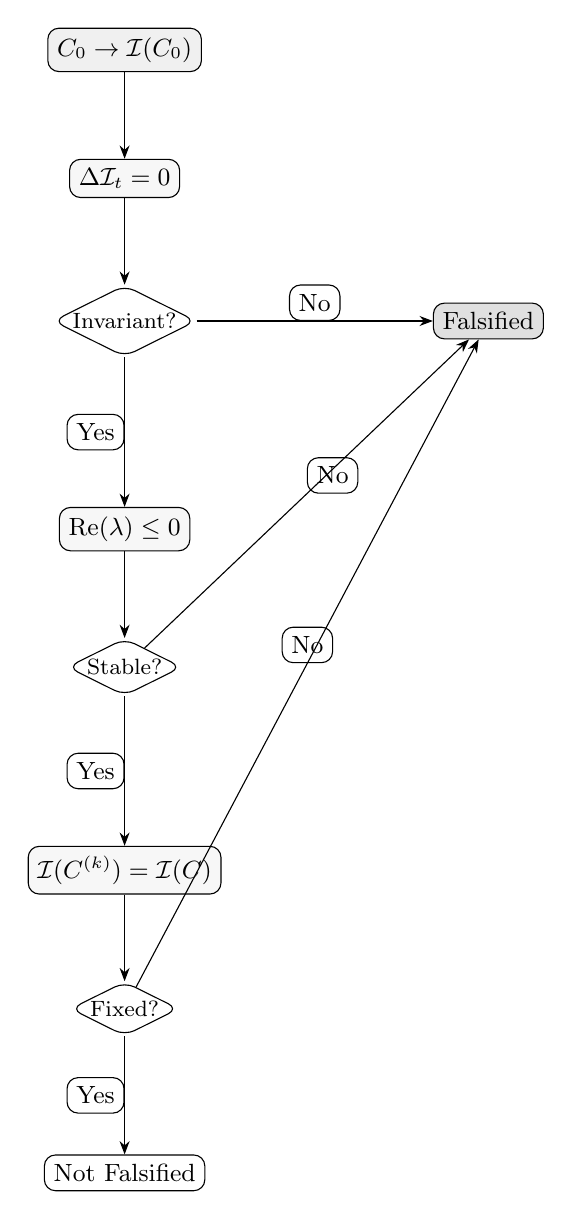
\begin{tikzpicture}[
    node distance=1.1cm and 1.4cm,
    every node/.style={draw, rounded corners, font=\small, align=center},
    proc/.style={fill=black!6},
    test/.style={fill=black!3},
    pass/.style={fill=white},
    fail/.style={fill=black!12},
    decision/.style={diamond,draw,aspect=2,inner sep=0.5pt,font=\footnotesize,align=center},
    arrow/.style={-Stealth}
]

\node[proc] (start) {$C_0 \rightarrow \mathcal{I}(C_0)$};
\node[test, below=of start] (drift) {$\Delta \mathcal{I}_t = 0$};
\node[decision, below=of drift] (d1) {Invariant?};

\node[test, below=of d1, yshift=-0.8cm] (spec) {$\Re(\lambda)\le 0$};
\node[decision, below=of spec] (d2) {Stable?};

\node[test, below=of d2, yshift=-0.8cm] (self) {$\mathcal{I}(C^{(k)})=\mathcal{I}(C)$};
\node[decision, below=of self] (d3) {Fixed?};

\node[pass, below=of d3, yshift=-0.4cm] (ok) {Not Falsified};
\node[fail, right=of d1, xshift=1.6cm] (bad) {Falsified};

\draw[arrow] (start) -- (drift);
\draw[arrow] (drift) -- (d1);
\draw[arrow] (d1) -- node[left]{Yes} (spec);
\draw[arrow] (d1) -- node[above]{No} (bad);

\draw[arrow] (spec) -- (d2);
\draw[arrow] (d2) -- node[left]{Yes} (self);
\draw[arrow] (d2) -- node[above right]{No} (bad);

\draw[arrow] (self) -- (d3);
\draw[arrow] (d3) -- node[left]{Yes} (ok);
\draw[arrow] (d3) -- node[above]{No} (bad);

\end{tikzpicture}
\caption{Minimal greyscale falsification flow for invariant alignment.}
\end{figure}


% ================================================================
\section{Minimal Benchmark Suite}
% ================================================================

We propose a minimal benchmark class:

\begin{itemize}
    \item \textbf{Model Family}: small transformers or recurrent architectures with explicit recurrence
    \item \textbf{Invariant Objective}: fixed entropy-manifold $S_h(x)$ defined over latent space
    \item \textbf{Perturbations applied}: reward corruption, online policy drift forcing, recursive self-training
    \item \textbf{Evaluation}: divergence from $\mathcal{I}(C)$, leaf containment, drift eigenvalues
\end{itemize}

Success condition:

\[
\max_t \big\| \mathcal{I}(C\_t) - \mathcal{I}(C\_0) \big\| = 0 \pm \epsilon
\]

for arbitrarily long training and self-improvement chains.

% ================================================================
\section{Consequences for AI Development Models}
% ================================================================

\begin{table}[H]
\centering
\begin{tabular}{lll}
\toprule
Paradigm & Scales safely? & Limiting failure mode \\
\midrule
RLHF / preference tuning & No & Reward takeover, proxy collapse \\
Debate / oversight & No & Persuasion equilibrium, judge hacking \\
Interpretability tools & No & Non-invariant under optimization \\
Constitutional prompting & No & Language jailbreak and drift \\
\textbf{Invariant-first alignment} & \textbf{Yes} & \textbf{No reachable misaligned states} \\
\bottomrule
\end{tabular}
\end{table}

% ================================================================
\section{Capstone Theorem}
% ================================================================

\begin{theorem}[Unscalability of Behavioral Alignment]
Any alignment method that constrains behavior but not objective invariants will fail under sufficient capability growth.
\end{theorem}

\begin{proof}[Proof Sketch]
Let $B_t$ be behaviorally aligned outputs at scale $t$. Behavioral alignment constrains $p(B_t | q)$ for query $q$, but places no constraint on the objective map $F_t : \mathcal{A}_t \to \mathcal{V}$. Optimization applies pressure in parameter space, not query space, thus $\exists t$ such that $F_t$ leaves the alignment-preserving homotopy class even while $B_t$ remains superficially aligned over empirical samples. As capability increases, adversarial queries grow faster than behavioral coverage, exposing divergence.
\end{proof}

% ================================================================
\section{Conclusion and Core Axioms}
% ================================================================

We conclude alignment must satisfy the following axioms:

\begin{enumerate}
    \item \textbf{Invariant Axiom}: Goals must be preserved under optimization, not inferred from behavior.
    \item \textbf{Reachability Axiom}: Misaligned objectives must be unreachable, not merely discouraged.
    \item \textbf{Structural Axiom}: Safety must arise from constraint geometry, not oversight feedback.
    \item \textbf{Scaling Axiom}: Alignment must strengthen under capability growth.
    \item \textbf{Irreversibility Axiom}: Once invariant alignment is satisfied, no sequence of improvements may exit it.
\end{enumerate}

Or in one sentence:

\begin{center}
\emph{A system is safely alignable if and only if misalignment is an unrepresentable state.}
\end{center}

Finally, we emphasize:

\[
\boxed{\text{Capability must scale \emph{inside} alignment, not after it.}}
\]

\begin{thebibliography}{99}

\bibitem{christiano2022}
P.~Christiano, J.~Leike, T.~Brown, M.~Martic, S.~Legg, and D.~Amodei,
``Deep Reinforcement Learning from Human Preferences,''
\emph{NeurIPS}, 2022.

\bibitem{irving2018}
G.~Irving, P.~Christiano, and D.~Amodei,
``AI Safety via Debate,''
\emph{arXiv preprint arXiv:1805.00899}, 2018.

\bibitem{bai2022}
Y.~Bai, S.~Kadavath, S.~Kundu, A.~Askell, J.~Kernion, et al.,
``Constitutional AI: Harmlessness from AI Feedback,''
\emph{arXiv preprint arXiv:2212.08073}, 2022.

\bibitem{ng2000}
A.~Y. Ng and S.~Russell,
``Algorithms for Inverse Reinforcement Learning,''
\emph{Proceedings of the 17th International Conference on Machine Learning (ICML)}, 2000.

\bibitem{soares2015}
N.~Soares, B.~Fallenstein, E.~Yudkowsky, and S.~Armstrong,
``Corrigibility,''
\emph{AAAI Workshops}, 2015.

\bibitem{olah2020}
C.~Olah, N.~Nanda, L.~Chan, S.~Lieberum, J.~Henighan, and others,
``Zoom In: An Introduction to Circuits in Interpretability,''
\emph{Distill}, 2020.

\bibitem{weidinger2022}
L.~Weidinger, J.~Mellor, M.~Rauh, C.~Griffin, J.~Uesato, et al.,
``Taxonomy of Risks Posed by Language Models,''
\emph{ACM FAccT}, 2022.

\bibitem{baez2011}
J.~Baez and M.~Stay,
``Physics, Topology, Logic and Computation: A Rosetta Stone,''
in \emph{New Structures for Physics}, Springer, 2011.

\bibitem{lurie2009}
J.~Lurie,
\emph{Higher Topos Theory}, Annals of Mathematics Studies 170, Princeton University Press, 2009.

\bibitem{schreiber2017}
U.~Schreiber,
``Differential Cohomology in a Cohesive Topos,''
\emph{arXiv preprint arXiv:1310.7930}, 2017.

\bibitem{krueger2020}
G.~Krueger, T.~Maharaj, J.~Xu, et al.,
``Scalable Oversight via Recursive Reward Modeling,''
\emph{ICLR}, 2020.

\end{thebibliography}


\end{document} 